%\section{Results and Discussions}
\begin{figure*}[htb!]
    \centering
    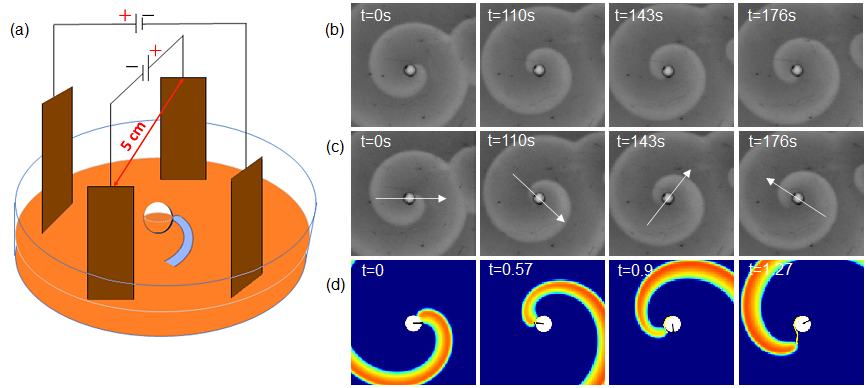
\includegraphics[scale=0.7]{new_fig.png}
    \caption{\textbf{(a) Schematic diagram of the experimental system:} The
	positions of two pairs of field electrodes with respect to the glass
	bead are shown schematically (not to scale).  \textbf{Unpinning of an
	anti-clockwise rotating spiral using CPEF:}  (b) An ACW rotating spiral
	pinned to a spherical bead of diameter 1.2 mm in the experiment. The
	natural period of pinned spiral tip $T_{s} = 297 $ s. (c) A CPEF of
	strength $E_0 \simeq 1.38$ V/cm, and period $T_{E} = 125$ s applied to
	the medium unpins the spiral tip from the obstacle. 
    (d) An ACW rotating spiral pinned to an obstacle of diameter 1.0 s.u in the
	simulation with $T_{s} = 1.77$ t.u is subjected to a CPEF of strength
	$E_0 \simeq 0.6 $ and period $T_{E} =1.18$ t.u. The spiral tip unpins
	from the obstacle at t = 1.27 t.u.  The arrows show the direction of
	the applied CPEF.}
    \label{fig:unpinning_images}
\end{figure*}
The rotating chemical wave in the BZ reaction medium can get anchored into the
boundary of the glass bead and form a very stable pinned wave, as shown in
Fig.~\ref{fig:unpinning_images}~b.  A similar situation occurs in the
numerical simulation of the model equations, where the spiral wave can get
anchored to the obstacle in the domain. It is known that this wave can be
unpinned with an electric field~\cite{Amrutha,???}. 
Here we employ the circularly polarized electric field (CPEF) using two
cross-electrodes, as described before. The CPEF can unpin the wave if the
amplitude of the electric field is above a certain threshold value ($E_{th}$),
as shown in Fig.~\ref{fig:unpinning_images}~c.  An arrow indicates the direction of the electric
field. Similar unpinning
is also seen in the model equations(Fig.~\ref{fig:unpinning_images}~d). To
understand the unpinning process, we measure the location at which the wave
leaves the obstacle. We can quantify the spiral location by the phase of the
spiral tip on the obstacle boundary. The phase is the angle of
the spiral tip, measured in degrees from the $+x$-axis along the anticlockwise
direction. The phase of the spiral when we start the CPEF is denoted by
$\phi_0$ and the phase when the spiral leaves the boundary is denoted by
$\phi_u$. The instantaneous direction of the electric
field is denoted by the angle $\theta_E$. The direction of the spiral
is along the tangent at the obstacle, and this direction is denoted by
${\hat{r}}_{t}$.  


\begin{figure}[htb!]
    \centering
    \includegraphics[width=\columnwidth]{cpef_phi0.png}
    \caption{\textbf{Unpinning at $E = E_{th}$:} 
     The phase difference (${\phi}_u$- ${\phi}_0$) is plotted against
	${\phi}_0$ for $p$ = 0.5 (underdrive pacing). (d) same as (c) but for
	$p$ = 1.5 (overdrive pacing). The condition where our unpinning
	condition repeats itself a second time is indicated by the dashed line.
	Circles and triangles represent the experiment and simulation data
	respectively.  
    %Note: Remaining experimental data will be added later.
    }
    \label{fig:unpinning_EthA}
\end{figure}
\begin{figure}[htb!]
    \centering
    \includegraphics[width=\columnwidth]{cpef_p.png}
    \caption{\textbf{Unpinning at $E = E_{th}$:} 
	For spirals having different
	${\phi}_0$,  the phase difference (${\phi}_u$- ${\phi}_0$) is plotted
	with the pacing ratio, p in (a) experiments and (b) simulations. At
	overdrive pacing ($p>$1), the red dashed lines on the top marks the
	theory curve for ${\phi}_0$=$315^0$ , corresponding to the second
	angular positions satisfying the unpinning mechanism. The solid red
	line at the bottom corresponds to the first set of angular positions
	satisfying the unpinning mechanism for ${\phi}_0$=$315^0$.
	}
    \label{fig:unpinning_EthB}
\end{figure}
In the experiments and simulations, we observe that the unpinning phase
depends linearly on $\phi_0$, as shown in Fig.~\ref{fig:unpinning_EthA}. The
unpinning angle also depends on the chirality of the spiral, the frequency of
CPEF. We define the pacing ratio, $p$, as the ratio of the frequency of the
CPEF($\omega_{cp}$) to that of the spiral($\omega_s$), {i.e.,} \( p=
\frac{\omega_{cp}}{\omega_{s}}\). We have varied $p$ from ??? to 4, as above 4
the field has no effect(???). Figure~\ref{fig:unpinning_EthB} shows unpinning
angle as a function of $p$ for various initial conditions in the experiments
and the simulations. It is seen that unpinning fails as $p$ approaches 1, for
most values of $\phi_0$. 

These results can be analyzed in light of our recent work with DC
electric fields~\cite{Amrutha}. We found that the electric field exerts a
retarding force on the chemical wavefront, which is maximum when the
field direction is along the direction of the wavefront. The direction of the
wavefront here is the direction of the tangent vector at the spiral tip. For a
CPEF this condition is satisfied when 
\begin{eqnarray}
	\phi_u &=& \frac{p \phi_0+ 90}{p-1} ; p>1 \\
	\phi_u &=& \frac{270-p \phi_0}{1-p} ; p<1  
\label{eq:Eth}
\end{eqnarray}

The theoretical solid curves in Figs.~\ref{fig:unpinning_EthA} and
\ref{fig:unpinning_EthB} are based on the above equation.   

When $p$=1, the condition for unpinning is met only for a small range of initial
conditions. When $E=E_{th}$, the wave can be unpinned only when the
$\theta_E-\phi_0 = 90$. For all other initial phases, the wave cannot be unpinned using CPEF.  
Following the mechanism at E = $E_{th}$, the unpinning for a field strength
greater than $E_{th}$ must occur when the component of $\vec{E}$ along
$\hat{r_t}$ reaches the critical threshold, $E_{th}$. i.e, when the scalar
product of ${\vec{E}}$ and ${\hat{r}}_{t}$ is equal to or greater than
$E_{th}$. This condition gives a window of possible spiral unpinning phase
$\phi_{u}$ in terms of $\phi_{0}$, p, E and $E_{th}$ as described below.

For overdrive pacing with $p>1$, the unpinning phase window is given by
\begin{equation}
\frac{p \phi_0+ {\sin^{-1}}(\frac{E_{th}}{E})}{p-1}   \leq \phi_u \leq \frac{p \phi_0+\pi -{\sin^{-1}}(\frac{E_{th}}{E})}{p-1}
\label{eq:overdrive}
\end{equation}
with a width $\Delta\phi_u = \frac{\pi - 2 \sin^{-1}(\frac{E_{th}}{E})}{p-1}$.
As the field vector begins to align parallel to the direction of spiral wave,
the unpinning condition (Eq.~\ref{eq:overdrive}) is satisfied at the lower
bound of this range. However, when $\phi_0$ falls within this range, the wave
unpins with a fixed delay, as observed with the DC electric field. (??? Some times it misses unpinning and has to come back; How do we demonstrate this?).
%To demonstrate these result, we plot ($\phi_u-\theta_E$) as a function of $\phi_0$
%in Fig.~\ref{fig:unpinningE>Eth}. Note that $\phi_u$  shows little variation
%when $\phi_0$ is outside the range given by Eq.~\ref{eq:overdrive}.


For underdrive pacing i.e, for $p<1$, the unpinning phase window is 
\begin{equation}
\frac{\pi+ {\sin^{-1}}(\frac{E_{th}}{E})-p \phi_0}{1-p}   \leq \phi_u \leq \frac{2\pi-p \phi_0-{\sin^{-1}}(\frac{E_{th}}{E})}{1-p}
\label{eq:underdrive}
\end{equation}
The width of this window is $\Delta\phi_u = \frac{\pi - 2 \sin^{-1}(\frac{E_{th}}{E})}{1-p}$. 


%%%%%%%%%%%%%%%%%%%%%%%%%%%%%%%%%%%%%%%%%%%%%%%%%%%%%%%%%%%%%%%%%%%%%%%%%%%%%%%%%%%%%%%%%%%%%%%%%%%%%%%%%%%%
For p = 1, unpinning happens only if the following condition is satisfied.
\begin{equation}
\pi+ \sin^{-1}(\frac{E_{th}}{E})  \leq \phi_0 \leq 2\pi-\sin^{-1}(\frac{E_{th}}{E})
\label{eq:p=1}
\end{equation} 
Thus for $p=1$ the range of initial phases that lead to
unpinning increase with the field strength, $E$. Fig.\ref{fig:E_p1}a shows the initial spiral
phases that lead to successful unpinning as a function of $\frac{E_{th}}{E}$.


%
\begin{figure}[htb!]
    \centering
	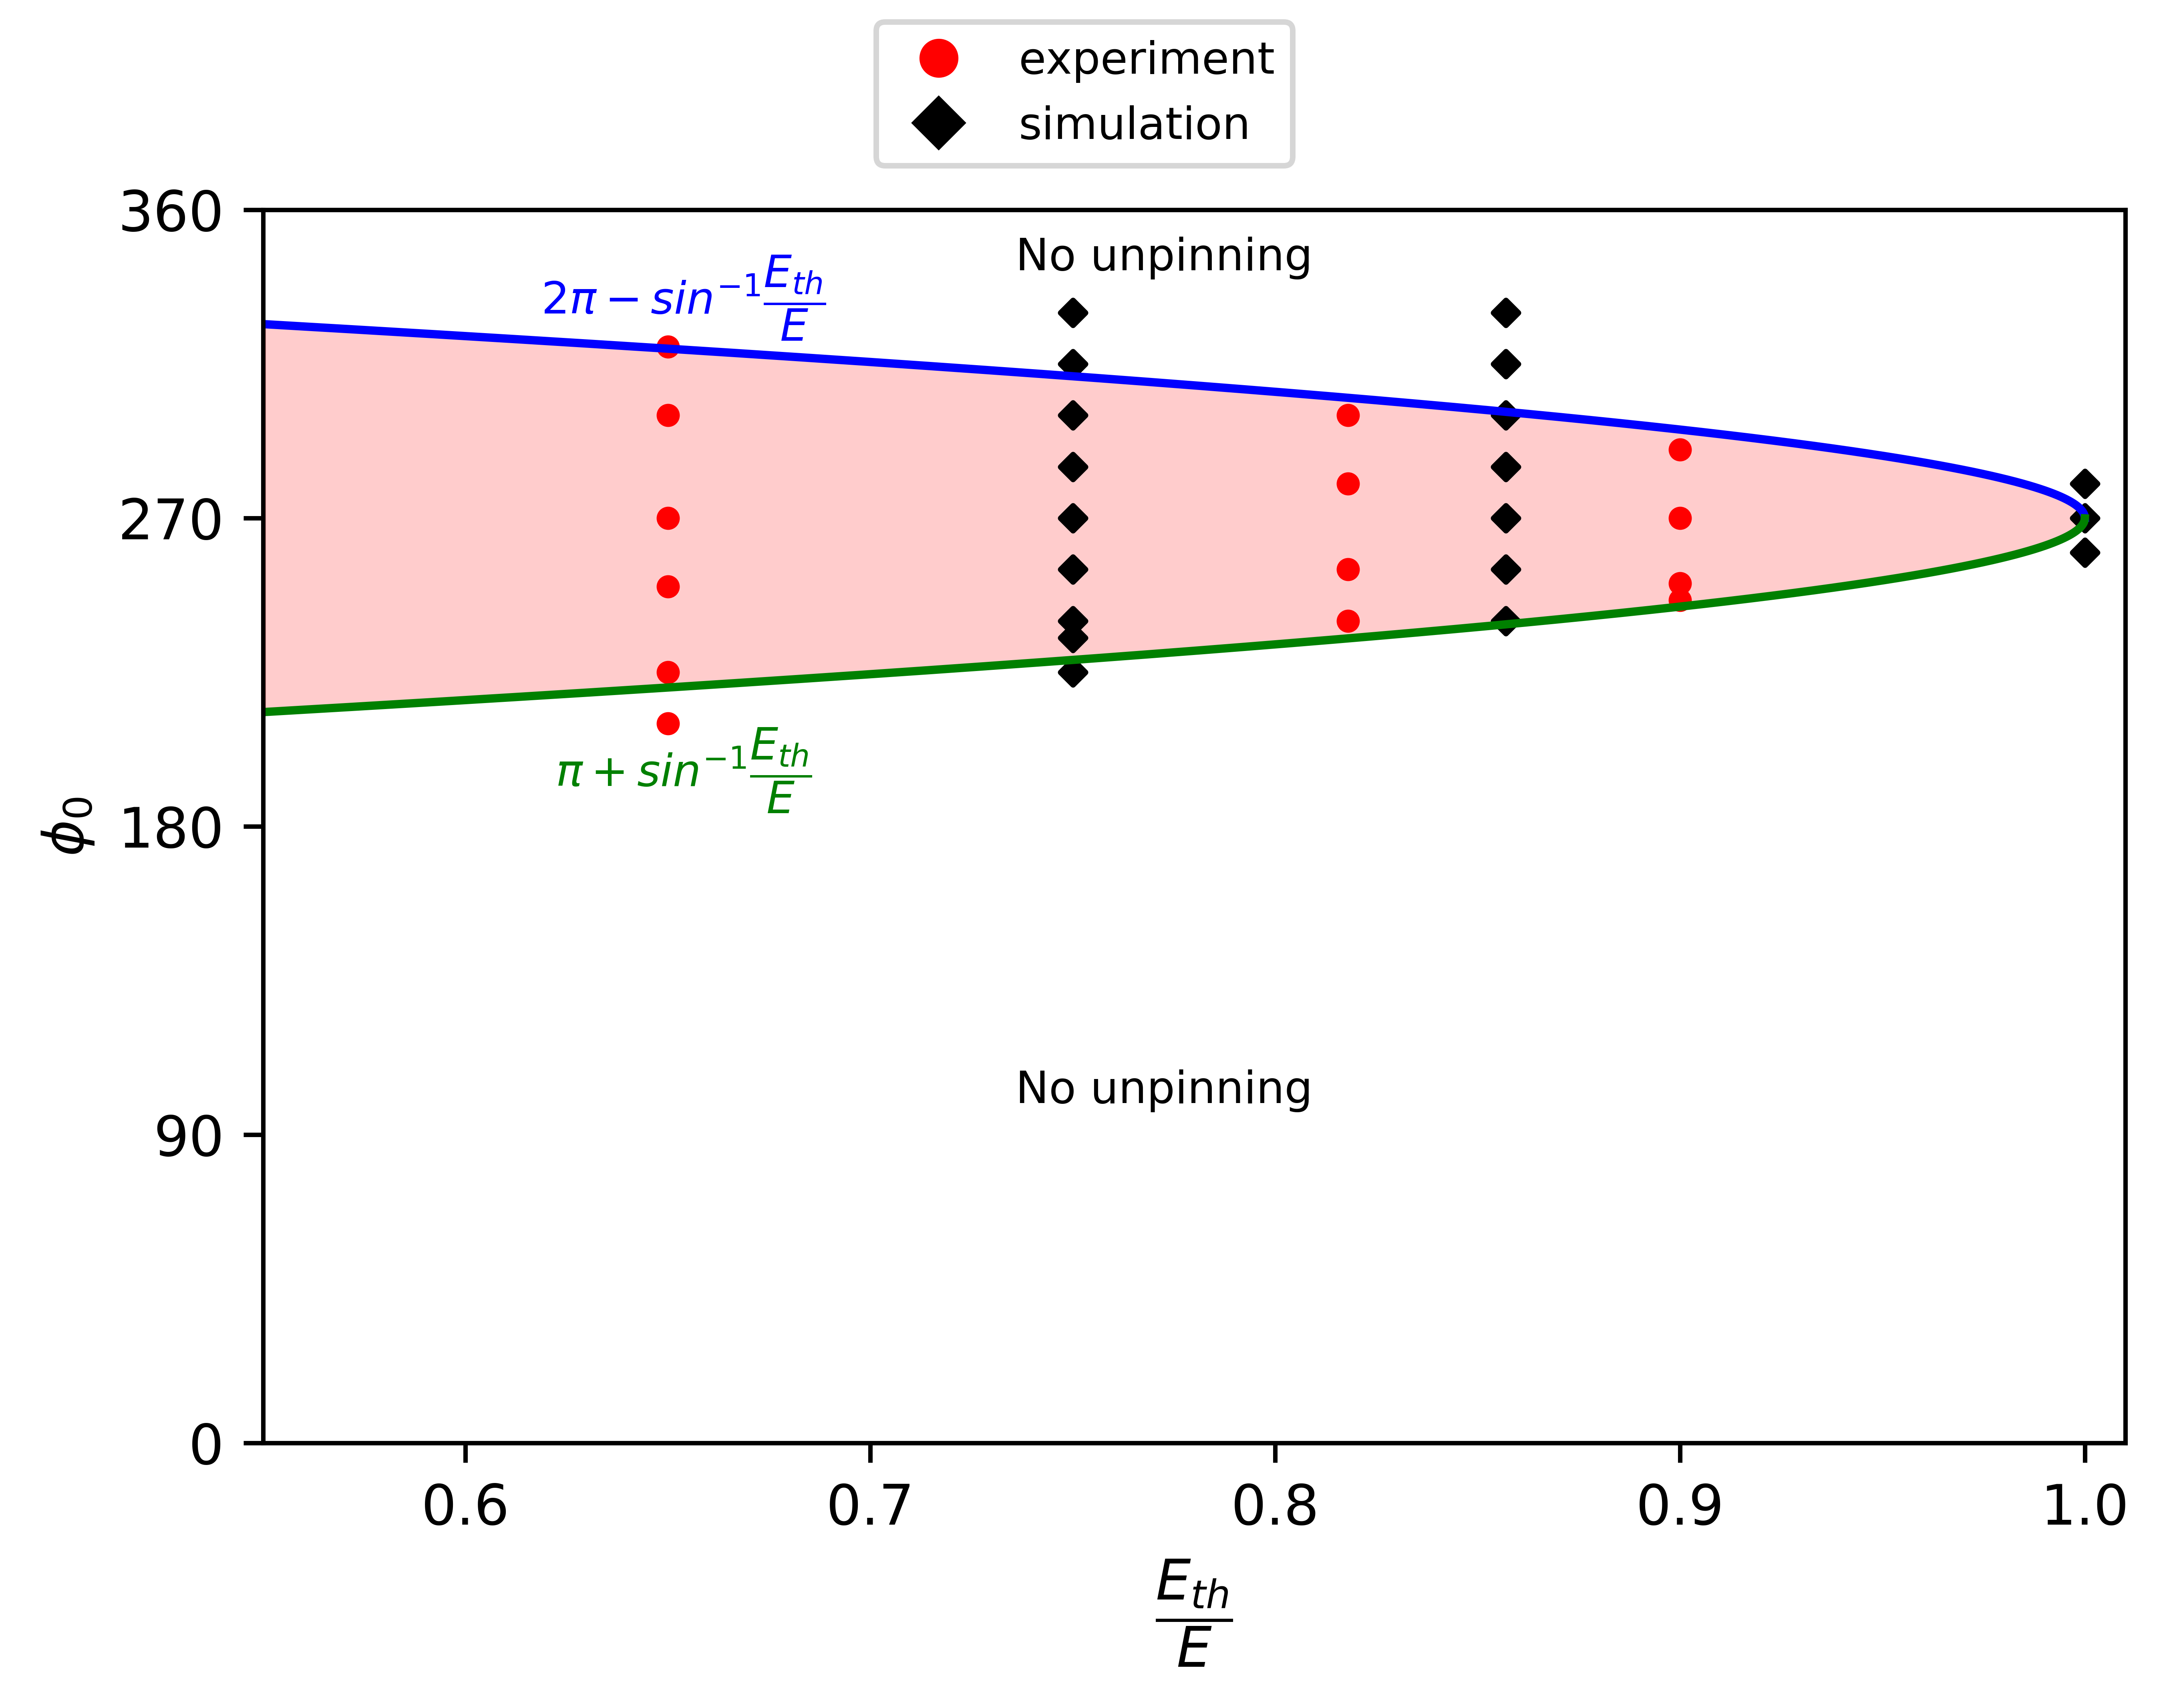
\includegraphics[width=\columnwidth]{p1.png}
    \caption{Unpinning of spiral wave with pacing ratio, p = 1 for different
	field strength: $\pi+{\sin^{-1}}{(\frac{E_{th}}{E})}$ and
	$2\pi-{\sin^{-1}}{(\frac{E_{th}}{E})}$ are the lower and upper limit of
	the range of possible ${\phi}_0$-values which gives successful
	unpinning for p = 1. Shaded region corresponds to the cases of
	successful unpinning.
    Circles and diamonds represent the experiment and simulation data
	respectively.} 
	\label{fig:unpinning_p1}
\end{figure}
%%%%%%%%%%%%%%%%%%%%%%%%%%%%%%%%%%%%%%%%%%%%%%%%%%%%%%%%%%%%%%%%%%%%%%%%%%%%%%%%%%%%%%%%%%%%%%%%%%%%%%%%%%%%%
%For p = 1, unpinning happens only if the following condition is satisfied.
%\begin{equation}
%\pi+ \sin^{-1}(\frac{E_{th}}{E})  \leq \phi_0 \leq 2\pi-\sin^{-1}(\frac{E_{th}}{E})
%\label{eq:p=1}
%\end{equation} 
%Thus for $p=1$ the range of initial phases that lead to
%unpinning increase with $E_{th}$. Fig.\ref{fig:E_p1}a shows the initial spiral
%phases that lead to successful unpinning as a function of $\frac{E}{E_{th}}$.



%%%%%%%%%%%%%%%%%%%%%%%%%%%%%%%%%%%%%%%%%%%%%%%%%%%%%%%%%%%%%%%%%%%%%%%%%%%%%%%%%%%%%%%%%%%%%%%%%%%%%%%%%%%

